% Instructions to modify this document:
% * Remember to ALWAYS execute "git pull" BEFORE any commit you make!
% * Use the \ToDo{...} command to remark tasks which still need to be done. Add your name in the comment.
% * Use the \input{file.tex} command to split the document into several parts
% * Do not change the current LaTeX coding style to yours. The style and format should be homogeneous along sections.

% To convert .dia diagrams into PDF:
% 1) Create the diagram with dia
% 2) Export it as .eps
% 3) use epstopdf to convert to PDF


\documentclass[a4paper,12pt]{article}

\usepackage[utf8]{inputenc}
\usepackage{amsmath,graphicx}
\usepackage{bm}
\usepackage{amssymb}
\usepackage{algorithm}
\usepackage{algpseudocode}
\usepackage{subfigure}
\usepackage{ifpdf}
\usepackage{url}
\usepackage{color}
\usepackage[hidelinks]{hyperref}
\usepackage{multirow}
\usepackage{datetime}
\usepackage{comment}
\usepackage{float} % To put figures in their exact place with \begin{figure}[H]
\usepackage{longtable}
\usepackage{tabularx}
\usepackage{listings}
\usepackage{xcolor}


\newcolumntype{L}[1]{>{\raggedright\arraybackslash}p{#1}}
\newcolumntype{C}[1]{>{\centering\arraybackslash}p{#1}}
\newcolumntype{R}[1]{>{\raggedleft\arraybackslash}p{#1}}


% Definitions and commands
\def \np{\vskip 0.25 cm}
\def \ap{\vskip 0.15 cm}

% JSON listing (see 
%  http://tex.stackexchange.com/questions/83085/how-to-improve-listings-display 
% -of- json-files)
\colorlet{punct}{red!60!black}
\definecolor{background}{HTML}{EEEEEE}
\definecolor{delim}{RGB}{20,105,176}
\colorlet{numb}{magenta!60!black}

\lstdefinelanguage{json}{
    basicstyle=\footnotesize\ttfamily,
    numbers=left,
    numberstyle=\scriptsize,
    stepnumber=1,
    numbersep=8pt,
    showstringspaces=false,
    breaklines=true,
    frame=lines,
    backgroundcolor=\color{background},
    literate=
     *{0}{{{\color{numb}0}}}{1}
      {1}{{{\color{numb}1}}}{1}
      {2}{{{\color{numb}2}}}{1}
      {3}{{{\color{numb}3}}}{1}
      {4}{{{\color{numb}4}}}{1}
      {5}{{{\color{numb}5}}}{1}
      {6}{{{\color{numb}6}}}{1}
      {7}{{{\color{numb}7}}}{1}
      {8}{{{\color{numb}8}}}{1}
      {9}{{{\color{numb}9}}}{1}
      {:}{{{\color{punct}{:}}}}{1}
      {,}{{{\color{punct}{,}}}}{1}
      {\{}{{{\color{delim}{\{}}}}{1}
      {\}}{{{\color{delim}{\}}}}}{1}
      {[}{{{\color{delim}{[}}}}{1}
      {]}{{{\color{delim}{]}}}}{1},
}


\newcommand{\ToDo}[1]{\textcolor{magenta}{\textbf{[ToDo]} \textbf{#1}}}
\newcommand{\miguel}[1]{\textcolor{magenta}{\textbf{[Miguel]} \textbf{#1}}}


\begin{document}


\begin{titlepage}

\begin{center}
\vspace*{-1in}

\vspace*{0.6in}
\begin{Large}
\textbf{The IPOL Demo System 2.0 \\Technical documentation} \\
\end{Large}

\vspace*{0.6in}

\small{Compiled on \today\ at \currenttime}

\vspace*{0.6in}
\rule{80mm}{0.1mm}\\
\vspace*{0.1in}
\end{center}

\end{titlepage}

This document contains technical documentation for the IPOL Demo System 2.0. Specifically, the architecture of the service-oriented platform, its modules, and the real-time template generation of demos from their textual description.
\vspace*{0.6in}

\textbf{Software engineers and external consultats, past and present (in alphabetical order):}


Martín Arévalo

José Arrecio

Miguel Colom

Joan Duran

Carlos Escobar

Vincent Firmin

Karl Krissian

José Luis Lisani

Alexis Mongin

Nelson Monzón

\vspace*{0.2in}

\textbf{Project direction and team coordination}

Miguel Colom - \url{http://mcolom.info}



%\maketitle
\newpage

\tableofcontents
\newpage
\listoffigures
\newpage

% The Archive module
\section{Introduction}
\ToDo{Incomplete section!}

The system is built as a service-oriented architecture \cite{neuman2015building}.
The functionality is decomposed into a set of independent, self-contained microservice modules which communicate with each other via an API.

By splitting the monolithic application into smaller modules and decoupling interdependencies (between apps, dev teams, technologies, environments, and tooling), the system gains in terms of scalability, parallel development, easier debugging, and complexity isolation.

\begin{figure}[!ht]
\centering
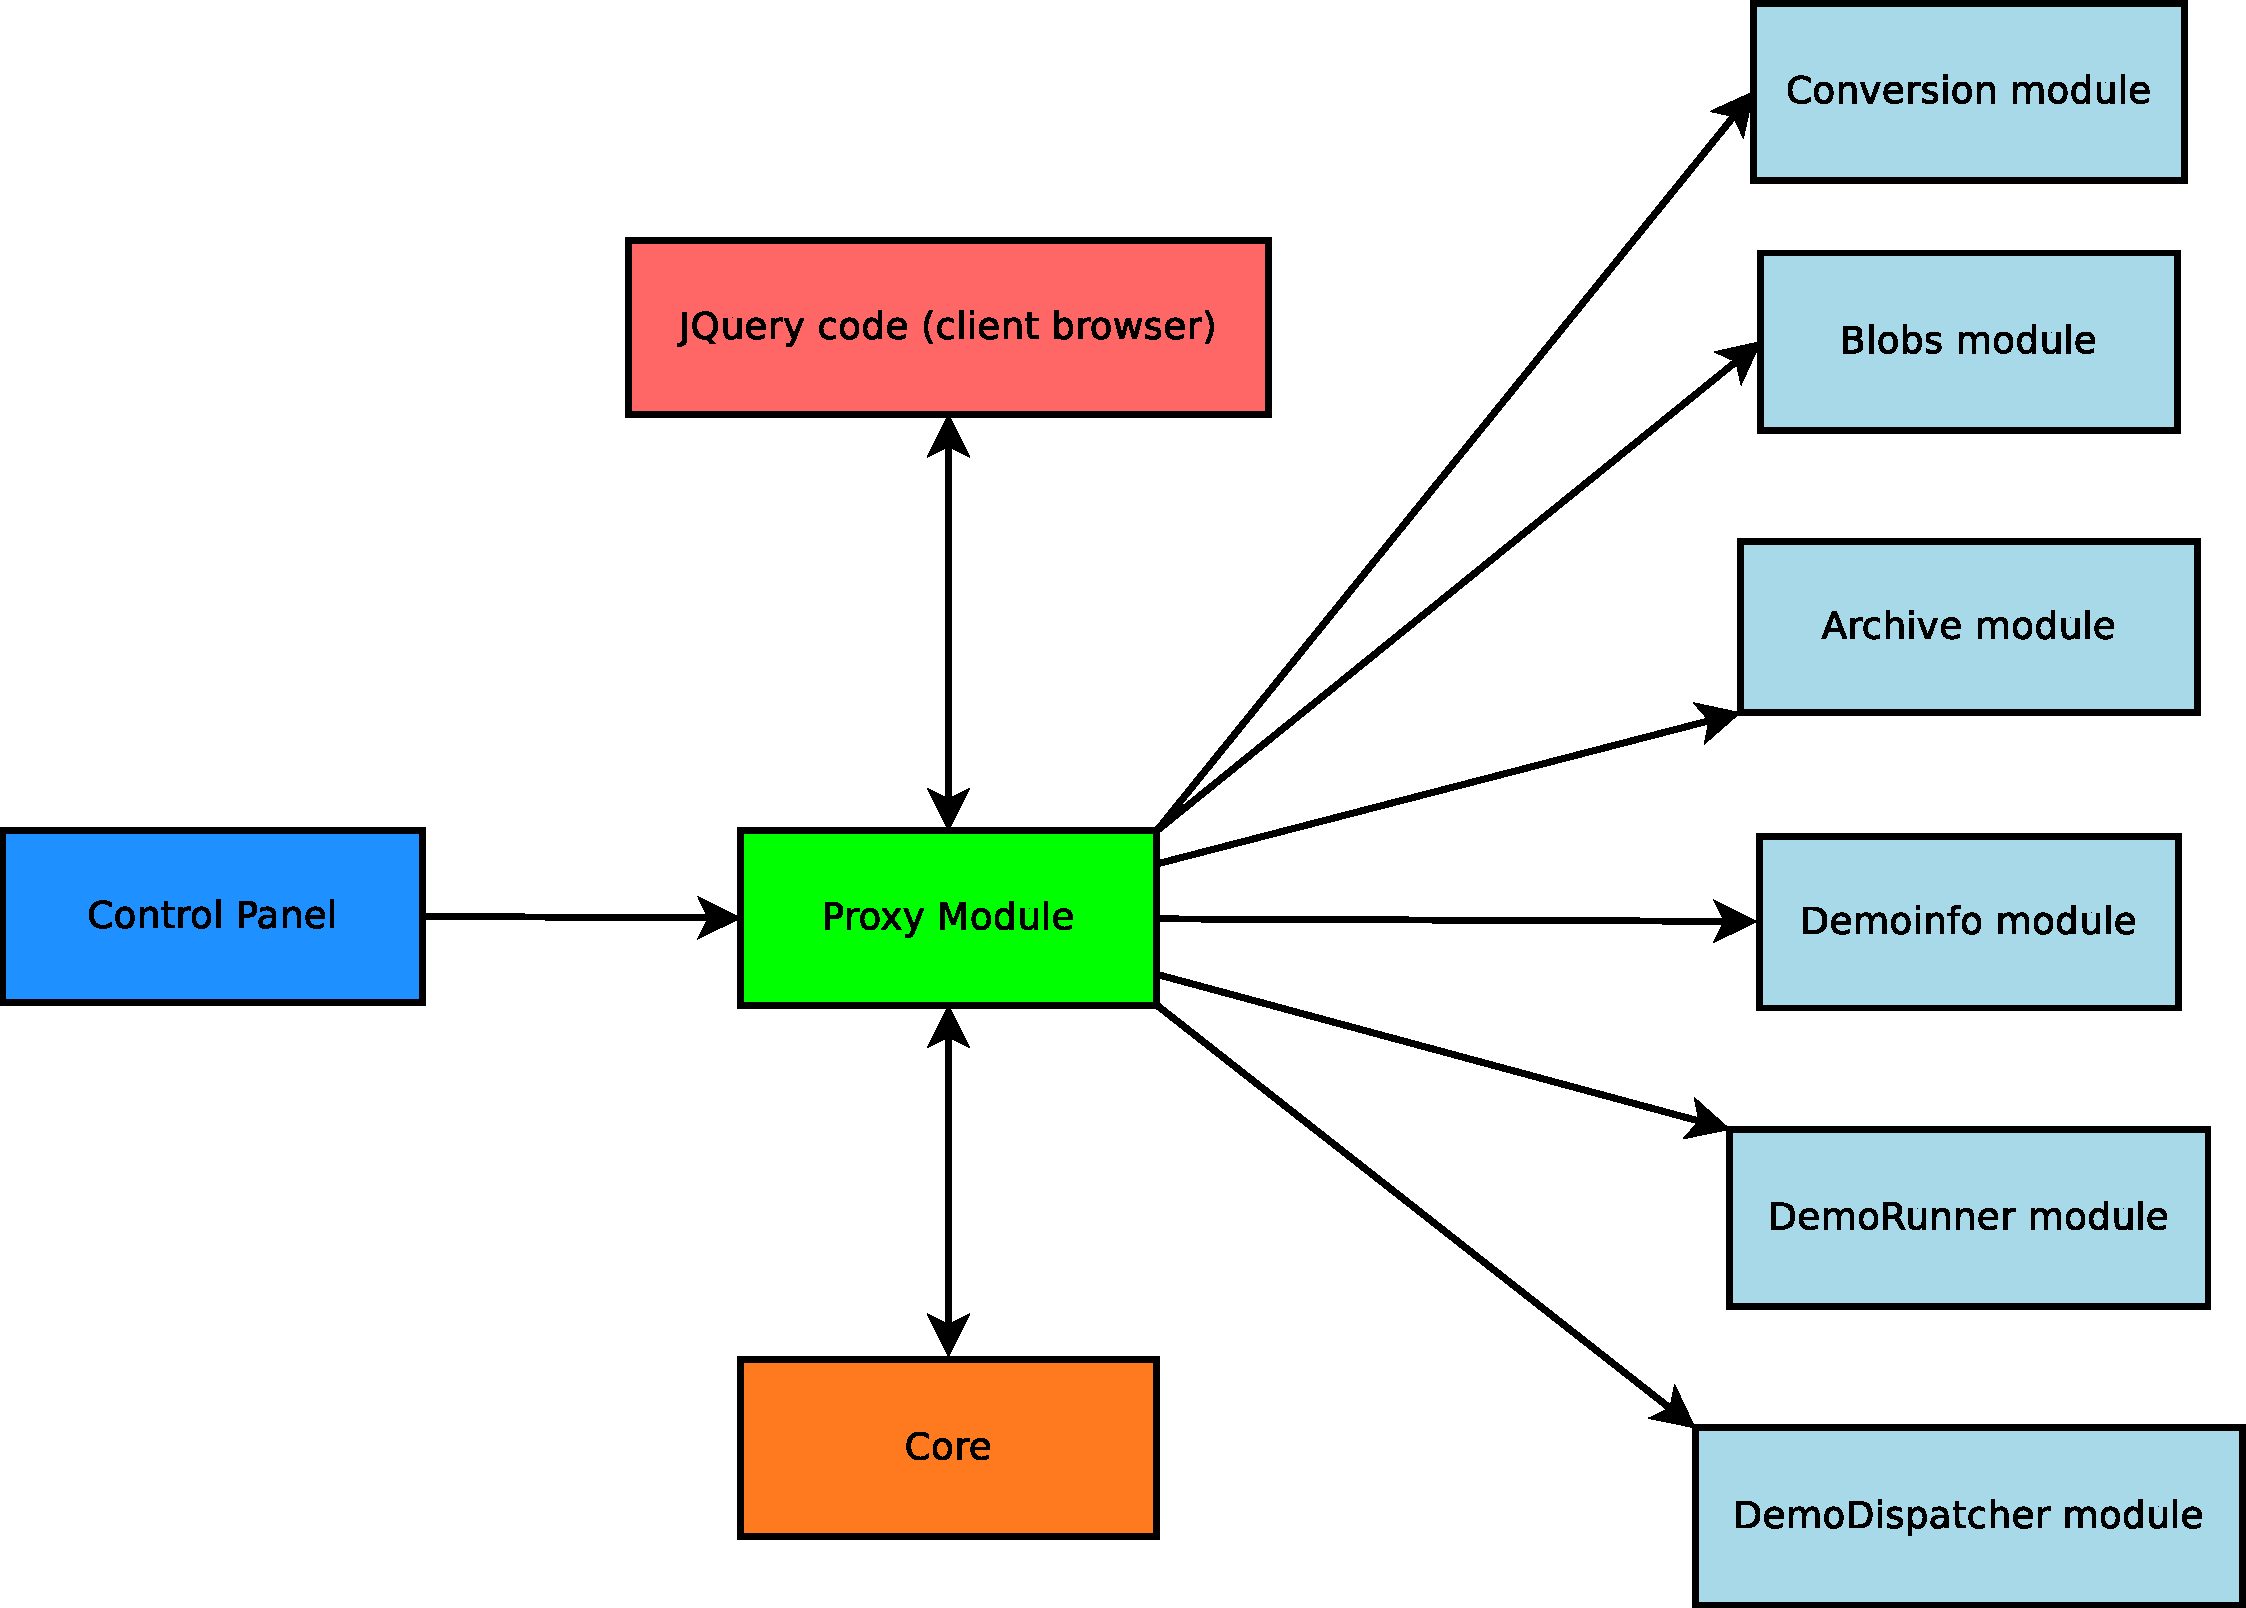
\includegraphics[width=0.8\linewidth]{architecture/images/architecture.pdf}
\caption{Modular system architecture.} 
\label{fig:architecture}
\end{figure}


% The Core
\section{The Demo System Core}
\ToDo{
OLD text. 
Centralized webservice.
The list of datatypes used (images, audio, video, 3D pointclouds, 3D meshes) and how to identify them. The "no type" format for demos which have their own non-standard format.}

In this section we explain the demo system core, that is the responsible of the coordination of the other modules. One of its main issues is controlling the execution of the different experiments. Figure \ref{fig:core_diagram} shows a diagram that explains the modules and the messages passed when executing an experiment.

The core performs very simple actions like creating the directories, copy the blobs for the experiment, etc, for ensuring that everything is ready for a demo execution. It delegates in the Demo Dispatcher module (see Sect.\ref{sec:DemoDispatcher}) the selection of the computer for the experiment. 

In order to distribute the load in several machines, this module checks the work load of each known DemoRunner modules (see Sect.~\ref{sec:DemoRunner}) and starts an algorithm demo execution on the less loaded machine. It uses a FIFO queue as a ``buffer'' to wait for a computer free to execute the demo and encapsulates an object to establishes the balancing policy that decides whether a process can leave the queue or not. Finally, the core uses the selected machine and waits until the experiment is finished. When it is finished, the core send to the archive module (see Sect.~\ref{sec:archive}) a JSON message for storing the experiment information.


\begin{figure}[!ht]
\centering
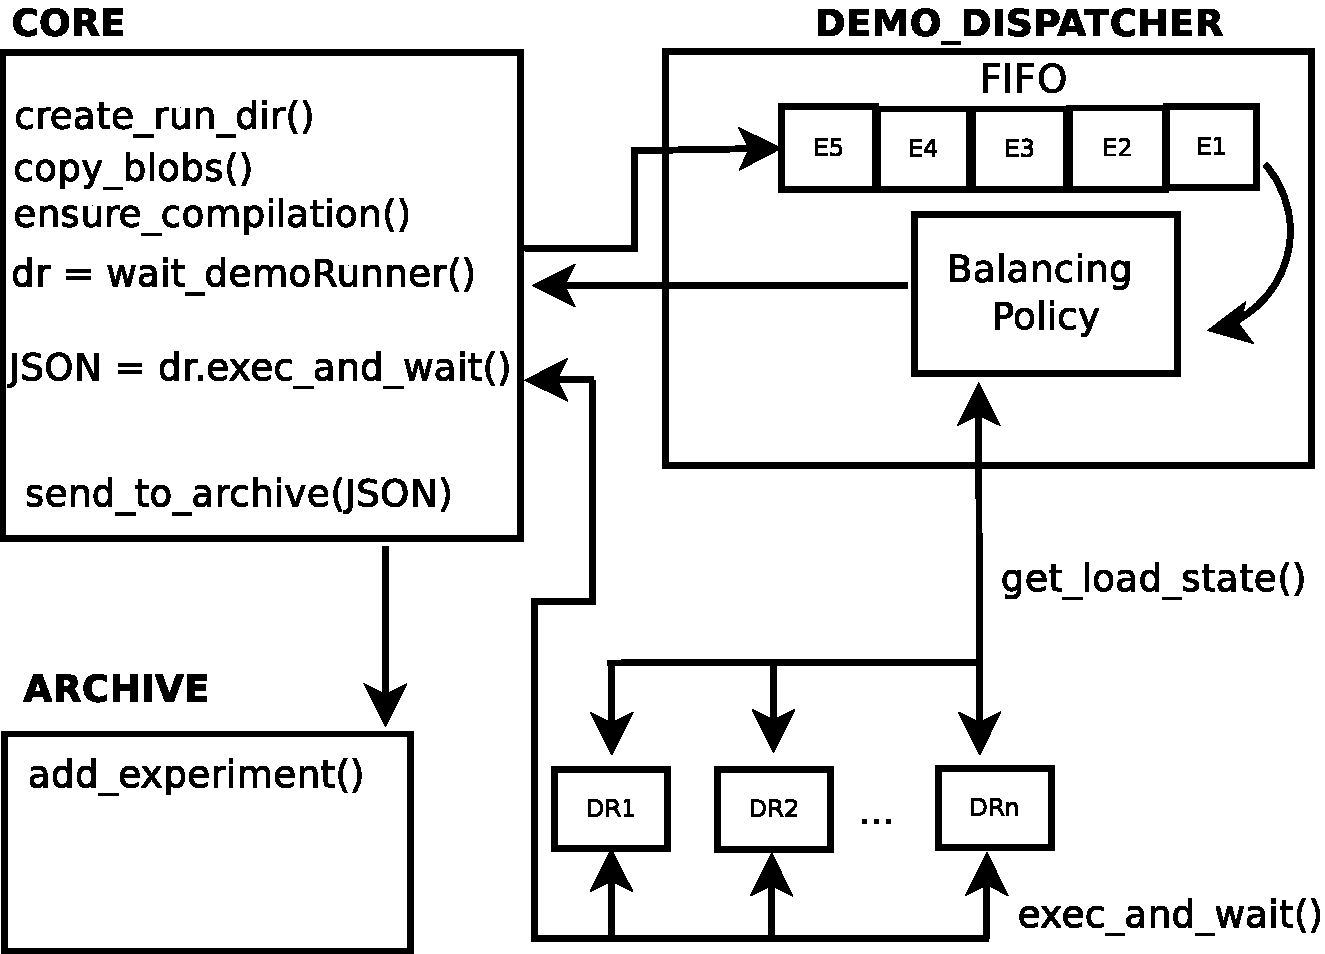
\includegraphics[width=0.7\columnwidth]{core/images/core_diagram.pdf}
\caption{Representation of the IPOL demos execution system.} 
\label{fig:core_diagram}
\end{figure}


\ToDo{Document it!}


% The Proxy module
\section{The Proxy module}

\subsection{Introduction}
\label{sec:proxy_introduction}

%~\cite{GoF}
Next, we explain the main features of the Proxy module. Its purpose is providing a correct and transparent communication between the different modules that composes the IPOL system. 

This proxy simplifies problems, such as the strong dependence between the machines where are located the other modules. For instance, if we want to change the location of one of our IPOL modules, we only need to modify the information file used in the proxy. As consequence, the system will not need more modifications for a correct performance.

\paragraph{Technologies used} \hspace{0pt} \\
The module is written in Python and uses the Cherrypy framework. The other modules must communicate with the proxy using a correct URL (see Fig.~\ref{fi:url_protocol}) while the output returns a JSON message.

\subsection{Architecture}

\paragraph{Module composition} \hspace{0pt} \\
The module is composed of the following files: the code itself in: ``proxy.py'', a main file for initiating the module: ``main.py''  and a cherrypy configuration file: ``proxy.conf''.  
It also uses a logs file for storing information when something is wrong using the proxy. This is initialised with the Proxy object using the logs directory provided in ``proxy.conf''.

\paragraph{Module architecture} \hspace{0pt} \\

The module is composed of a class, named as 'Proxy', that encapsulates all the information needed by the proxy. The services offered by the module are all methods of this class. The cherrypy framework provide the abstraction for making the methods available as webservices. 

The cherrypy engine is launched when the module starts. Besides, it loads the cherrypy configuration from “proxy.conf”. It also creates (if not exist) a logs folder using the information from the cherrypy configuration file and stores all the modules information provided by the XML file as a dictionary.

When other module requests a service, it must communicate with the proxy using arguments given through an URL. The latter must follow a few guidelines. If the requesting module does not fulfill well with the required specifications, the proxy returns a JSON message that notifies the error and writes it in the file “error.log” in the logs directory

\subsection{Communication with the proxy}

In this section, we explain how the modules must communicate with the proxy for requesting a web service. They must input their petitions by using the following protocol for the URL:
\begin{figure}[!ht]
\centering
\begin{verbatim}
http://<proxyUrl>:<port>/?module=<module>&service=<ws>
&parameters=<ws_parameters>
\end{verbatim}
%\caption{Url protocol for a correct use of the proxy.} 
\label{fi:url_protocol}
\end{figure}

%At the moment, the URL and the port of the proxy are: \\ \texttt{http://ns3018037.ip-151-80-24.eu:9003/}. \\
In this sense, an example of the how to use the proxy for requesting a web service is:

\begin{figure}[!ht]
\centering
\begin{verbatim}
http://ns3018037.ip-151-80-24.eu:9003/?module=archive&
service=ping
\end{verbatim}
\label{fi:url_ping_example}
\end{figure}

If the module does not use this protocol or something goes wrong, the proxy rejects the petition, writes the error in the log file and returns a JSON string to notify, using a code number, the reason of the failure (see table~\ref{ta:codes}). On the other hand, when the petition succeeded, the proxy outputs the JSON message from the requested web service. \\

The JSON format of the proxy reads as follows:
\begin{figure}[!ht]
\centering
\begin{verbatim}
{
    status : KO
    url_parameters: Number of parameters introduced in the URL
    code: Flag indicating the reason of the failure
}
\end{verbatim}
\end{figure}


\begin{table}[tbp]
\centering
\begin{tabular}{|c|c|}
\hline
\textbf{Code} & \textbf{Mean} \\
\hline
 0   & URL without parameters \\
\hline
-1   & The URL does not fulfill the protocol  \\
\hline
-2   & 
\begin{tabular}{c}
Parameter for the module empty or  \\
the proxy does not recognize it
\end{tabular}
\\
\hline
-3   & Web service not specified. \\
\hline
-4   & 
\begin{tabular}{c}
An error in the communication \\
(for example, the requested module is down)
\end{tabular}
\\
\hline
-5   & Error from the requested module \\
\hline
\end{tabular}
\label{ta:codes}
\caption{Codes determining the type of error when using the proxy module} 
\end{table}

\ToDo{Document it!}


% The Blobs module
\section{The Blobs module}

Note: to avoid confusion, we refer the modules of the IPOL system as ``ipol modules'' and Python modules (files containing Python code) as ``Python modules''.

\subsection{Introduction}
Each demo of IPOL offers the user a set of defaults blobs. Thus, the users are not forced to supply their own files for the executions of the algorithms. These defaults blobs can be tagged and linked to differents demos.

\subsection{Composition}
The blobs module is composed of several Python modules. It is composed of the same technical stack as the rest of the rest of the IPOL modules: written in Python, using a web server, a database, and using templates for generating HTML responses for webservices destinated to humans.

\subsubsection{Main Python module}
The main module is called by ``start.sh'', the script called by the control terminal to get modules running on different servers over ssh. It consist of setting up some variables used by cherrypy, as well as mounting the blobs class at the root of the used server.

\subsubsection{Error Python module}
This module describes the errors issued by the Blobs IPOL module and adds color to the error messages printed in the terminal.

\subsubsection{Database and database Python module}
The first and most important design constraint of the Blobs IPOL module was that data shouldn't be duplicated. All blobs referenced by multiple demos should exist in only one directory. This is addressed by establishment of one relational database, referencing the demos, the blobs, and the relationship between them. This database also permits to tag some text on blobs, as well as organize them in named sets. In the big picture, the database Python module a implement a simple CRUD\footnote{Acronym for Create, Read, Update, Delete. These operations allows the total manipulation and the persistancy of data inside a data structure.} interface for manipulating the database. Blobs can be managed individually, and upon the deletion of a demo, the blobs related to this demo will be deleted from disk if and only if they were uniquely linked to this demo. Blobs are referenced via their hashes, making it easy to verify if a blob is already in the database, even under another filename. \\

\begin{figure}[h]
\centering
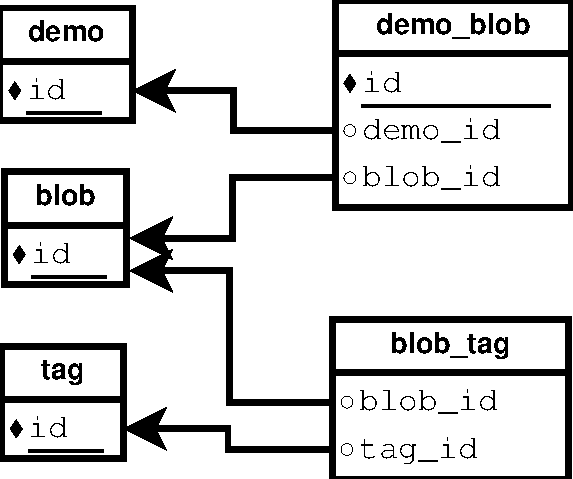
\includegraphics[scale=0.75]{blobs/images/blobs_database.pdf}
\caption{The database architecture of the blobs module} 
\label{fig:blobs_database}
\end{figure}


In the figure~\ref{fig:blobs_database}, id fields are the primary keys (it is worth noting that the primary key of a blob\_tag entry is the combination of the foreign keys it contains), the other fields are foreign keys, and the arrows indicate which primary keys are referenced by which foreign keys.
Three tables, demo, blob and tag, contains the information about referenced demos, blobs, and tags relating to blobs. Two junction tables link this information together, referencing the blobs standards to a demo, and the tags owned by each blobs.

\paragraph{The database Python module\\}
This module offers an interface for accessing the database. One object of the class Database should be instanciated for each operation modifying it. Even if it has function for connecting and closing, they should not be used as such, for flow control issues (for example, an exception leaving a connection open). A very simple abstraction, the DatabaseConnection class is present in the blobs Python module for it, and allow safe connection to the database, ensuring they will always be closed no matter what.

Otherwise, this Python module offer us a wide variety of simple methods for interacting with the database, or obtaining metrics of it, such as the total number of blobs. They generally return the information asked if such case apply. For the format of the responses and the different function, we refer the reader to the code of the module itself. It is worth noting that one webservice, delete\_blob\_from\_demo, recompute the positions of the blobs in a set in which a blob was deleted. If this function is accessed concurrently by multiple threads (the most likely case is if a webservice calling this function is accessed several times in a very short span), the blobs can end up with miscalculated positions. Non-concurrential access should be enforced by locking the scope where this webservice is called. Such a lock is used in the delete\_blob\_ws webservice in the blobs Python module.

\subsubsection{Blobs module}
The blobs Python module is the core of this. It implement three classes, DatabaseConnection as referenced earlier in the present documentation, and MyFieldStorage, for intermediate storage of the uploaded blobs in the /tmp/ directory, and Blobs as an encapsulation of the webservices and the data they use. It also has some utilitary function.

The Blobs class implements all the webservices constituting this module, both those transmitting JSON to other modules, and those generating HTML via templates for humans. An instance of the Blobs class should possess information about the storage of blobs and the networking parameters cherrypy use, such as a port number. A cherrypy configuration file, named ``blobs.conf'' contains the informations one might need to change to run the module on another server, without changing the code, such as the directories where the blobs can be found, the port used by the cherrypy engine, or the path to the database.

The webservices of the module access the database via instanciations of Database objects managed by the DatabaseConnection class. Some read information, and some modify the database by adding or removing information. For handling a webservice automatically and charging his JSON response as a Python object, the utilitary function use\_web\_service is used.

Logging is utilized as a mean to retrieve the errors occuring in the system. The logger implemented in the blobs Python module handle all the errors of the module. It is passed to each Database object instanciation.

Here is a list of all the webservices implemented by the blobs module :

\begin{itemize}
\item default : The service invoked when asked for non-existing service.
\item index : web page at the root of where the module is mounted in cherrypy.
\item blob : web page used to upload one blob to one demo.
\item archive : Used to upload one zip file of compressed blobs to one demo.
\item add\_blob\_ws : service checking that the given blobs do not exist in the database. If this is the case, add it.
\item add\_blob : implement the add\_blob page.
\item demos\_ws : return the list of demos from the database.
\item get\_template\_demos\_ws : return the list of template demos from the database
\item demos : web page used to add a demo to the database.
\item set\_template\_ws : webservice used to change the template used by a demo.
\item use\_template : web page used to change the template used by a demo.
\item add\_demo\_ws : web service used to add a demo to the database.
\item add\_demo : web page used to add a demo to the database.
\item add\_from\_archive : webservice used to upload a zip file of compressed blobs to one demo.
\item add\_tag\_to\_blob\_ws : webservice used to add a tag to a blob.
\item op\_add\_tag\_to\_blob : web page used to add a tag to a blob.
\item remove\_tag\_to\_blob\_ws : webservice used to remove a tag from a blob.
\item op\_remove\_tag\_to\_blob : web page used to remove a tag from a blob.
\item op\_remove\_blob\_from\_demo : web page used to remove a blob from a demo.
\item get\_blobs\_from\_template\_ws : webservice used to get the list of blobs from templated demo.
\item get\_blobs\_of\_demo\_by\_name\_ws : webservice returning a list of the hashes of the blobs owned by given demo name.
\item get\_blobs\_of\_demo\_ws : same as the precedent, but with the demo id.
\item get\_blobs\_of\_demo : web page used to display blobs owned by a given demo.
\item edit\_blob : web page showing the thumbnail of a demo with the possibility to add or remove tags.
\item get\_blob\_ws : webservice returning information about a blob from its id.
\item get\_tags\_ws : webservice returning tags of a blob from its id.
\item op\_remove\_demo\_ws : webservice removing a demo from its id.
\item op\_remove\_demo : web page used for removing a demo.
\item ping : used by the terminal for checking module status.
\item shutdown : used by the terminal for turning off the module at distance.
  
\end{itemize}


% The Archive module
\section{The Archive module}

\subsection{Introduction}
\label{sec:archive_introduction}

%\paragraph{Introduction} \hspace{0pt} \\
The archive module is a standalone application destinated to communicate with other modules using webservices. It is designed to implement a stable, simple and scalable system for archiving all experiments done with IPOL.

\paragraph{Technologies used} \hspace{0pt} \\
The archive module is written in Python, is using the cherrypy framework for webservices, the mako template library for webpage rendering, the Python Image Library for thumbnails creations, and the python-magic library available on pip (not to be mistaken with python-magic5 which is the one available on default ubuntu's APT repositories). The module communicate using JSON, both in input and output. The database engine used is SQLite.

\subsection{Architecture}

\paragraph{Module composition} \hspace{0pt} \\
The module is composed of very few files, the code itself in ``module.py'', a cherrypy configuration file ``archive.conf'', two mako HTML templates, and a database. It will also need 4 directories, respectively for storing blobs, thumbnails, the database and logs.

\paragraph{Module architecture} \hspace{0pt} \\
The module is composed of a class, Archive, encapsulating the datas needed to function. The services offered by the module are all methods of this class. The cherrypy framework provide the abstraction for making available the methods as webservices. \\
Upon starting the module, the cherrypy engine is launched, an object of the Archive class is created, and the cherrypy configuration is loaded from ``archive.conf''. If they don't exists, both the database and the directories needed for the storage of blobs, logs, the database and thumbnails will be created, provided that the user launching the module has the necessary rights. Otherwise, the module will not start. These directories are indicated in the cherrypy configuration for maximum configurability, if they are missing from it, the module will not start. \\
The webservices communicate with the server via arguments given through URL, as unicode strings directly passed to the methods. \\
The services all connect to the database in a thread-safe way, instanciating its own connection when called, commiting when done if there is modifications, or rollbacking if there is an error, and closing the connection. \\
There is a logger initialised with the Archive object, writing errors in ``error.log'' in the logs directory given in the configuration file.

\subsection{Database design}

The database contains 3 tables : experiments, blobs, and correspondence.\\
Each experiments, and each blobs are defined individually, and linked to each-others in the correspondence table, assuring a many-to-many connection. It is worth noting that the database doesn't save duplicates of the same blob. \\

\begin{tabular}{|l|c|r|}
  \hline
  experiments & blobs & correspondence \\
  \hline
  id & id & id \\
  id\_demo & hash & id\_experiment \\
  params & type & id\_blob \\
  timestamp & format & name \\
  \hline
\end{tabular} \\

\paragraph{Experiments table} \hspace{0pt} \\
The experiments table is defined as such : the id field, that store the unique id of the experiment ; the id\_demo field, that store the id of the IPOL demo used for the experiment ; the params field, which is a JSON string whose format vary from demo to demo ; and finally the timestamp field.

\paragraph{Blobs table} \hspace{0pt} \\
The blobs table is defined as such : the id field, that store the unique id of the blob ; the hash field, that store the hash of the blob computed with sha1, the type field, that store the extension of the blob (exemple ``jpeg'' or ``png''), and the format field, that store the media format of the blob : it is a string, either ``audio'', ``video'' or ``image''. \\
The physical location of a blob is ``blob\_dir defined in configuration file'' + ``hash of the blob'' + ``.'' + ``type of the blob''.

\paragraph{Correspondence table} \hspace{0pt} \\
The correspondence table is defined as such : the id field ; the id of the experiment and the id of the blob that is linked to said experiment, and the name field, which indicate the role of the blob in the experiment (example : ``input'' or ``denoised''). A foreign key constraint allowing cascade delete is put on the field id\_experiment, referencing the id of an entry in the experiment table, for automatic data deletion.

\subsection{Services}

\paragraph{Adding an experiment to the archive} \hspace{0pt} \\
The method ``add\_experiment'' take in entry the id of the demo used ; a JSON string of the format : 

\begin{tabbing}
tabs \= tabs \kill
\{ \\
\>url\_blob : name\}, \\
\> ... \\
\} \\
\end{tabbing}

containing a description of each blobs used by and produced by the experiment, with their temporary URLs and names ; and a JSON string describing the parameters of the demo used for the experiment. It will add an experiment to the database by creating a new entry in the experiment table. If the blobs used by and produced by the experiment aren't already in the database, it will copy them in the directory given in the configuration file, and, for the images, create a thumbnail. It will return a json string containing the status of the operation, OK uf it succeeded, KO if there was an error and the operation wasn't performed, as such :

\begin{tabbing}
tabs \= tabs \kill
\{ \\
\>status : OK/KO\}, \\
\} \\
\end{tabbing}

If status is KO, a log describing the error will be written.

\paragraph{Deleting an experiment from the archive} \hspace{0pt} \\
When removing an experiment from the database via the method ``delete\_experiment'', every blobs linked to this experiment and only to this experiment are removed. After that, all the entries in the correspondence table referencing this experiment are removed automatically due to a foreign key constraint. It return a json response containing the status of the operation of the same format as the return of the method ``add\_experiment''.

\paragraph{Deleting a blob from the archive} \hspace{0pt} \\
Due to a many-to-many link between blobs and experiments in the database, a blob has a lot of dependencies : it has of course the experiments using this blobs, but also the blobs linked to these experiments. For deleting a blob from the archive, the precedent service is called on each experiment the blob is part of, assuring that no orphans datas stay in the database (for exemple, experiments linked to removed blobs or blobs linked to removed experiments). The method implementing this service is ``delete\_blob\_w\_deps''. It return a json response containing the status of the operation of the same format as the return of the method ``add\_experiment''.

\paragraph{Getting datas from an archive page} \hspace{0pt} \\
The method ``page'' return in a JSON response, for a given page of a given demo, all the datas of the experiments that should be displayed on this page. Twelve experiments are displayed by page. For rendering the archive page in the browser, the JSON response should be parsed and interpreted in a dedicated template furnished by the front-end of another module. The JSON response is formatted this way : 
\begin{tabbing}
tabs \= tabs \= tabs \= tabs \= tabs \= tabs \kill
\{ \\
\> status :  OK/KO, \\
\> experiments : [ \\
\> \> \{ \\
\> \> \> date : timestamp\_example, \\ 
\> \> \> files : [ \\
\> \> \> \>  \{ \\
\> \> \> \> \> url : url\_example, \\
\> \> \> \> \> id : id\_example, \\
\> \> \> \> \> name : name\_example, \\
\> \> \> \> \> url\_thumb : url\_thumbnail\_example \\
\> \> \> \> \} \\
\> \> \> ... ], \\
\> \> \> id : id\_example, \\
\> \> \> parameters = \{parameters\_example...\} \\
\> ... ], \\
\> id\_demo : id\_demo\_example, \\
\> nb\_pages : nb\_pages\_example \\
\} \\
\end{tabbing} 

\paragraph{User interface for removing blobs/experiments} \hspace{0pt} \\
The only user interface furnished by the archive module is for removing blobs or experiment in a convenient manner. It use the json response of the precedent service and render the ``archive\_admin\_tmp.html'' template displaying a page of archive for given demo, allowing the deletion of both blobs and experiments by simply linking to two other services calling deletion methods and updating the template. In case of error, for example when invalid datas are given through URL, ``error.html'' is rendered.

\paragraph{Shutdown} \hspace{0pt} \\
The method ``Shutdown'' shutdown the archive application when called. It return a json response containing the status of the operation.

\paragraph{Other services}
Other services features the method ``ping'', simply for checking if the module is up, and the method ``stats'', formatted this way :
\begin{tabbing}
tabs \= tabs \kill
\{ \\
\> status : OK/KO, \\
\> nb\_experiments : x, \\
\> nb\_blobs : y \\
\} \\
\end{tabbing}


% The Demo Info module
\section{DemoInfo module}
This module store the textual description of the demo and allows to ask for specific sections of it. It also stores other demo-related information, as:
\begin{itemize}
\item Demo id
\item Abstract
\item Title 
\item Autors list
\item Autors email list
\item Article URL
\item State (inactive,preprint, published)
\item Demo editor
\item Demo editor email
\item Demo zip file containing demo DDL 
\item Demo DDL Json
\end{itemize}

This module will be used by the controll panel module, the demo will be extracted from the zip file, it will be created in Demoinfo module, The blobs will be addede to Blobs module.

\subsection{ demoinfo module structure}
This Module is formed by:
\begin{itemize}
\item model.py where the db structure, the DAO (Data access object) clasess and some helper claseses (Demo, Authorand Editor) are defined. It provides a layer of abstarction over the DB.
\item demoinfo.conf it's the cherrypy config for the webservices module.
\item demoinfo.py it's the webservices module.
\item testdemoinfo.py it's the tests to chech that the webservices work.
\item testdemoinfo.conf it's the cherrypy config for testing.
\end{itemize}

\subsection{The model (database) structure}
The model of this module id formed by the following tables:

\begin{figure}[!ht]
\centering
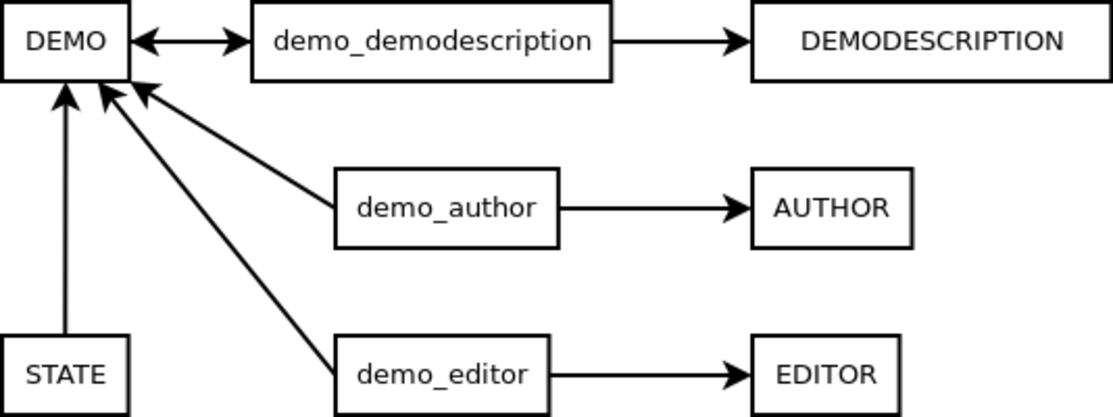
\includegraphics[width=0.5\columnwidth]{demo_info/images/demoinfo_model.pdf}
\caption{Demoinfo Database Model.} 
\label{fig:demoinfo_model}
\end{figure}

Note that states is the table for the demo's state (Published,preprint...)
Demodescription table is where the demo description language (DDL) for each demo is stored.
A demo may be created without a DDL (but you will need to provide one so you can run it)
Ddlschema is not used at the moment, but it has been created so that a schema validation can be done to the DDL of each demo, if a user provides a valid json for the DDL but this json is not a valid DDL , whe should be able to detect thisand return an error.

\subsection{Web services available}
This module provides a set of webservices, those that return data can be called with GET or other html methods, those that delete,create or update data can be called only by POST.
These webservices are shown grouped by functionality, 


DEMO

\begin{itemize}
\item  demo\_list(self)
\item  demo\_list\_by\_demoeditorid(self,demoeditorid\_list)
\item  demo\_list\_pagination\_and\_filter(self,num\_elements\_page,page,qfilter=None)
\item  demo\_get\_authors\_list(self,demo\_id)
\item  demo\_get\_available\_authors\_list(self,demo\_id)
\item  demo\_get\_editors\_list(self,demo\_id)
\item  demo\_get\_available\_editors\_list(self,demo\_id)
\item  demo\_get\_demodescriptions\_list(self,demo\_id,returnjsons=None)
\item  read\_demo\_metainfo(self, demoid)
\item  read\_demo\_metainfo\_by\_editordemoid(self, editordemoid)
\item  add\_demo(self, editorsdemoid, title, abstract, zipURL, active, stateID, demodescriptionID=None, demodescriptionJson=None)

Allows you to create a demo
- allow only post
- only creating the demo
- creating the demo and assigning an existing ddl (with id demodescriptionID) to it
- create the demo and create a ddl , whith the json passed by param (demodescriptionJson)

\item  delete\_demo(self,demo\_id,hard\_delete = False)
allow only post
\item  update\_demo(self,demo)
allow only post
\end{itemize}


AUTHOR

\begin{itemize}
\item  author\_list(self)
\item  author\_list\_pagination\_and\_filter(self,num\_elements\_page,page,qfilter=None)
\item  read\_author(self, authorid)
\item  author\_get\_demos\_list(self,author\_id)
\item  add\_author(self,name, mail)
allow only post
\item  add\_author\_to\_demo(self,demo\_id ,author\_id)
allow only post
\item  remove\_author\_from\_demo(self,demo\_id ,author\_id)
allow only post
\item  remove\_author(self,author\_id)
allow only post
\item  update\_author(self,author)
allow only post
\end{itemize}


EDITOR

\begin{itemize}
\item  editor\_list(self)
\item  editor\_list\_pagination\_and\_filter(self,num\_elements\_page,page,qfilter=None)
\item  editor\_get\_demos\_list(self,editor\_id)
\item  read\_editor(self, editorid)
\item  add\_editor(self,name, mail)
allow only post
\item  add\_editor\_to\_demo(self,demo\_id ,editor\_id)
allow only post
\item  remove\_editor\_from\_demo(self,demo\_id ,editor\_id)
allow only post
\item  remove\_editor(self,editor\_id)
allow only post
\item  update\_editor(self,editor)
allow only post
\end{itemize}

DDL

\begin{itemize}
\item  read\_demo\_description(self, demodescriptionID)
\item  read\_last\_demodescription\_from\_demo(self,demo\_id,returnjsons=None)
\item  add\_demodescription\_to\_demo(self,demo\_id, demodescription\_id)
allow only post
\item  add\_demo\_description(self,demoid=None,inproduction=None)
allow only post
\item  add\_demo\_description\_using\_param(self, demojson,inproduction = None)
\item  update\_demo\_description(self, demodescriptionID)
\end{itemize}

MISCELLANEA

\begin{itemize}
\item  index(self)
\item  ping(self)
\item  shutdown(self)
\item  stats(self)
\item  read\_states(self)
\end{itemize}


\subsection{Module testing}
To test this module enter test folder and run 
\begin{lstlisting}[language=Python,firstnumber=1]
python -m unittest discover.
\end{lstlisting}

To perfom manual testing use curl or poster pluguin for firefox (remember that some will only work with post requests) but in testdemoinfo.py, in the last tests you will find a working example of how to use some webservices using the request python library.
If you add webservices, please add the corresponding tests.

\ToDo{Secure access to Ws, oauth perhaps?}

% The Demo Dispatcher module
\section{DemoDispatcher module}
\label{sec:DemoDispatcher}
In order to distribute the load in several machines, this module checks the work load of each known DemoRunner modules and starts an algorithm demo execution on the less loaded machine. The process is done transparently and from the outside this is the only visible module, since the actual DemoRunners are not directly accesible.

It use a FIFO, that is a method of queuing process, for dispatching the different experiments. A machine for the demo runner sne

% \begin{algorithm}[!htbp]
% \caption{Dispatcher}
% \label{al:pyramidal_structure}
% \While{q not empty}
%     \State $ e_{i} \leftarrow q.extract()$
%     \State $ Dr = find\_dr()$
%     \State $ h = get\_id\_e(e_{i})$
%     \State $ notify_dequeue(h) $
%     \State $ Dr\_exec(e_{i}) $
%     \State $ Notify\_execution(h) $ 
% \EndWhile
% \end{algorithm}

\ToDo{Document it!}


% The Demo Runner module

\section{DemoRunner module}
\label{sec:DemoRunner}

This module controls the execution of the IPOL demos. It can execute directly its binaries or supporting scripts (provided by the demo editors) related to a particular demo (demoextras). Besides, a demo editor can use some generic scripts (PythonTools) that helps for representing the results of a demo such as draw 2D curves, draw histograms, counting lines and similar.

The DemoRunner intervines twice during an execution. First, this module is responsible of informing the Core about the load of the machine where it is running and ensuring that the demo execution is done with the last source codes provided by the authors (it downloads and compiles these codes to maintain them updated). Second, the Demorunner executes the algorithm with the parameters set by the users. It takes care of stopping the demo execution if a timeout is reached, and to inform the Core about the causes of a demo execution failure so the Core can take the best action in response. 

% The Control Terminal 
\section{The Control Terminal}

\subsection{Introduction}
The Control Terminal is a small application intended to system administrators which allows to start, stop, and query the status of each module. It is composed of an XML file describing each modules, and of the terminal itself, a python script. \\
Upon launch, a prompt will appear, asking the user for a command.

\subsection{Architecture}
The terminal allows the user to type a variety of commands, for controlling the states of each modules composing the IPOL system. Some take parameters, generally the name of a modules. Every command is coded in the terminal script, and the XML file list for every module, the commands that can be used with this module as parameter.

\paragraph{XML file} \hspace{0pt} \\
The XML file ``modules.XML'' is parsed at the beginning of the execution of the python terminal for storing a dictionnary describing each module. \\
For security purposes, it is important to stress that the IPOL system must be deployed in a way of making this file trusted input : a call to the system() function in the terminal using content of this file open the way to a shell remote exploit if someone were to modify it. \\
Each module is defined by the attribute ``name'' and contain a variable number of tags : ``url'', ``server'', and ``path'', each describing respectively the url where the services provided by the module can be accessed, the server where the module is, and the path to the modules directory on said server. After that, an undefined number of ``command'' tags allow the module to be given as parameter for said commands. In order to function, the commands start, ping and shutdown.

\paragraph{Structure of the dictionnary parsed from the XML file} \hspace{0pt} \\
The dictionnary has, as keys, the name of each modules, and as value, another dictionnary with the following keys : ``url'', ``server'', ``path'', ``commands''. All of them but ``commands'' take as value the strings in the XML file server. The last key, ``commands'', takes as value a list of strings, each being a command available to the module. This list contains every string in ``command'' tags in the XML file, plus the string ``info'', which is added automatically. This dictionnary is the only attribute of the terminal object, initiated as ``self.dict\_modules''.

\paragraph{Execution loop} \hspace{0pt} \\

Upon start of the terminal, a ``Terminal'' object is created, the XML file is parsed as described before, then the data is stocked in a dictionnary, as the state of the ``Terminal'' object. This state should not change during the execution. After that, a simple loop is iniated, asking the user for input, evaluating said input and printing the result. For parsing the input, an entry buffer is used, with as key, the strings corresponding to the commands, and as value, the function executing said command (one could argue, the command itself). The input string is split in a list of words, the separation character being the space or `` ``. Then, the first word is given to the entry buffer for determining the function the user want to call, and the rest of the list is passed as parameter, allowing the retrieval of the parameters in the commands functions. \\
The loop repeat until an EOF indicator is encountered or if the input string is ``exit''. As such, ``exit'' is not a command, and no call to the exit syscall are being made, not allowing for exiting with a given value. \\
The terminal doesnt possess features such as pipes, redirections and multiples commands given in one input.

\subsection{Commands}

\paragraph{start} \hspace{0pt} \\
Usage :
\begin{verbatim}
start <module>
\end{verbatim}
The ``start'' command tale a module as parameter, ssh into the server where the module is located, and launch the module using its file start.sh. The command ``ping'' should be launched after for checking if the module is up.

\paragraph{ping} \hspace{0pt} \\
Usage :
\begin{verbatim}
ping <module>
\end{verbatim}
The ``ping'' command take a module as parameter, and call a webservice for checking if the module is up.

\paragraph{shutdown} \hspace{0pt} \\
Usage :
\begin{verbatim}
shutdown <module>
\end{verbatim}
The ``shutdown'' command take a module as parameter, and call the webservice for this module to shutdown.

\paragraph{info} \hspace{0pt} \\
Usage :
\begin{verbatim}
info <module>
\end{verbatim}
The ``info'' command take a module as parameter, and print the list of available commands for this module.

\paragraph{modules} \hspace{0pt} \\
Usage :
\begin{verbatim}
modules
\end{verbatim}
The ``modules'' command display a list of the modules.

\paragraph{help} \hspace{0pt} \\
Usage :
\begin{verbatim}
help
\end{verbatim}
The ``help'' command print the help of the terminal.




\section{System administration}
\ToDo{This section is just a stub for the moment. Add all the system administration and configuration stuff here}

- Backups. For the moment we use the very simple script at {\tt ipolDevel/sysadmin/backup.sh}
Cron controls it. To add the cron line, use {\tt crontab -e} as root.

The format of the crontab lines is: minute (m), hour (h), day of month (dom), month (mon), and day of week (dow), or use '*' in these fields (for 'any').

For example, to run the backup script once per week at 3:00h, add this line:

{\tt 0 3 * * 1 /home/ipol/ipolDevel/sysadmin/backup.sh}

- Cleanup. The script {\tt ipolDevel/sysadmin/cleanup.sh} does a cleanup of all temporary files older than one month. To execute each month, the following line needs to be added with {\tt crontab -e} as root.

{\tt 0 5 * * 1 /home/ipol/ipolDevel/sysadmin/cleanup.sh}

- PyLint report. The script {\tt ipolDevel/ci\_tests/pylint.sh} uses PyLint to create code quality reports. It executes weekly in the integration server and sends an email to the addresses in the file {\tt send\_to.txt}

To execute each month, the following line needs to be added with {\tt crontab -e} as root.

{\tt 0 15 * * 2 sudo -u ipol /home/ipol/ipolDevel/ci\_tests/pylint.sh}

- pdflatex report. The script {\tt ipolDevel/ci\_tests/pdflatex.sh} checks if the Latex documentation of the project compiles and sends and email otherwise.

To execute each month, the following line needs to be added with {\tt crontab -e} as root.

{\tt 0 15 * * 2 sudo -u ipol /home/ipol/ipolDevel/ci\_tests/pdflatex.sh}



\subsection{GitHub deploy key}
The IPOL GitHub repository might be private. Thus, is any server needs to obtain the complete source code of the demo system, a \emph{deploy key} is needed. The deploy key is added to the GitHub configuration and each server needs to get the sources using the deploy key.

For example:

\begin{verbatim}
ipol@smartalgo:~/ipolDevel$ cat ~/.ssh/config 
host github_deploy
      hostname github.com
      user git
      identityfile ~/.ssh/id_rsa
\end{verbatim}

\vspace{0.15cm}

\begin{verbatim}
ipol@smartalgo:~/ipolDevel$ cat ~/.ssh/config 
host github_deploy
      hostname github.com
      user git
      identityfile ~/.ssh/id_rsa

ipol@smartalgo:~/ipolDevel$ cat .git/config 
[core]
	repositoryformatversion = 0
	filemode = true
	bare = false
	logallrefupdates = true
[remote "origin"]
	#url = https://github.com/mcolom/ipolDevel
	url = git@github_deploy:mcolom/ipolDevel.git
	fetch = +refs/heads/*:refs/remotes/origin/*
[branch "master"]
	remote = origin
	merge = refs/heads/master
\end{verbatim}

We use the host \emph{github\_deploy} in order to pick the deploy key in the SSH connection.

\subsection{Setup of a new machine}
When a new machine is added to the IPOL infrastructure, the following needs to be done:
- Create the {\tt ipol} user in a new machine: {\tt adduser --disabled-password ipol}

- Install bash-completion {\tt apt-get install bash-completion}

- Install cron-apt: {\tt apt-get install cron-apt}

And edit /etc/cron-apt/config:
\begin{verbatim}
APTCOMMAND=/usr/bin/apt-get
OPTIONS="-o quiet=1 -o Dir::Etc::SourceList=/etc/sources.list"
SYSLOGON="always"
\end{verbatim}

- Configuration of the email server to be able to send emails form any of the IPOL servers: configure with {\tt dpkg-reconfigure exim4-config} and be sure to choose the option to send email on the Internet, not local.

Install mail with {\tt apt-get install mailutils}

To send an email: {\tt cat email.txt | mail -s "This is the subject" john.doe@example.com,banania.guy@example.com}


- Setup priorities and memory limits to the processes of the users.

Added this to /etc/security/limits.conf:
\begin{verbatim}
*               soft     priority            17
ipol            soft     priority            0
\end{verbatim}

We need to set also limits for the memory usage per user. It'd be great if we could do it as a percentage of the free memory.


%To limit the memory which a group of users can use, we should use {\tt cgroups} along with the {\tt Cgred} daemon.
%
%More info:
%
%\url{https://www.digitalocean.com/community/tutorials/how-to-limit-resources-using-cgroups-on-centos-6}
%
%\url{https://access.redhat.com/documentation/en-US/Red_Hat_Enterprise_Linux/6/html/Resource_Management_Guide/sec-Moving_a_Process_to_a_Control_Group.html}



\section{General notes}
In this section we add general comments on the projects, parts which still neeed to be written or coded. In general, information which needs to be documented but has not still found its place in the document. It works as a reminder not to forget.

\begin{itemize}
  \item The magic module. We use PIP, not the python-magic package found in most distributions. \ToDo{Explain why}.
  \item List of packages needed and how to install them.
  \item Description of the general requirements needed for a module to be part of the system (start, ping, and shutdown services ; structure of the general launching script...
\end{itemize}

- List of packages used for installing the system. Packages to be installed with sudo apt-get install:

\begin{itemize}
\item python2.7
\item wget: to download files
\item cmake: to create a multiplatform Makefile easily
\item libtiff5-dev libtiff-tools libjpeg-dev libpng-dev: open and write TIFF, JPEG, PNG files
\item libfftw3-dev: fast DFT operations
\item libgsl0-dev libeigen3-dev liblapack-dev libblas-dev: linear algebra
\item python python-dev python-cherrypy3 python-mako python-jsonschema: Python language, Python headers, webserver, web templating, JSON
\item gnuplot gnuplot-nox: to draw figures
\item python-pip: to install python packages
\item python-yaml: for parsing
\item libpq-dev: PostgreSQL headers
\item libmagic-dev: needed to install python-magic with pip
\item libav-tools: audio/video tools for demos with these data types
\item gsl-bin libgsl0-dev  libblas-dev libblas3 libatlas-base-dev libatlas3-base liblapack-dev liblapack3: numerical computations with GSL, BLAS, LAPACK
\end{itemize}

Packages to be installed with pip install:
\begin{itemize}
\item python-magic
\item pillow
\item simplejson
\item validoot (\url{https://github.com/AstromechZA/validoot/tarball/1.3})
\end{itemize}

- Example of another demo system: \url{http://places.csail.mit.edu/demo.html}

- Integrate Openseedragon, \url{https://openseadragon.github.io/}

- Document the format of the demo package, with desc.jon, images/, extra/, etc

- Most of our modules name the files according to the hash sum of their contents. This file names are OK for internal use, but the users should obtain the files with the proper names. This can be achieved with the ``download" attribute in HTML5. All website interfaces should provide the corresponding human-readable name. For example:

\begin{verbatim}
<a href="9021384984901238490128490123841222223312.png" download="denoised.png">
  Download the denoised image
</a>
\end{verbatim}

- Look for potential race conditions everywhere in the code, specially at the modules. Use locks to prevent them.

- All webservices should return a \emph{status:KO} when they fail. For example, if they're asked a service which doesn't exist they should return the status:KO, but never simply return a cherrypy message because of an untreated exception. Example of a wrong behavior:

\begin{verbatim}
http://ns3018037.ip-151-80-24.eu:9002/hello

404 Not Found

The path '/hello' was not found.

Traceback (most recent call last):
  File "/usr/lib/python2.7/dist-packages/cherrypy/_cprequest.py", line 670, in respond
    response.body = self.handler()
  File "/usr/lib/python2.7/dist-packages/cherrypy/lib/encoding.py", line 217, in __call__
    self.body = self.oldhandler(*args, **kwargs)
  File "/usr/lib/python2.7/dist-packages/cherrypy/_cperror.py", line 411, in __call__
    raise self
NotFound: (404, "The path '/hello' was not found.")
Powered by CherryPy 3.5.0
\end{verbatim}

- In general, check that no FK reference is missing at any of the database schemas of the modules, and that they're correct.
Also, we need to check absolutely that all the CASCADE DELETE are correct!

- FYI: the package \emph{sqlitebrowser} seems to be a very good tool to browse and develop the SQLite schemas.

- The demoInfo module returns \emph{Content-Type: text/html} instead of application/json:

\begin{verbatim}
curl --head http://ns3018037.ip-151-80-24.eu:9002/read_demo_description?demodescriptionID=359
HTTP/1.1 200 OK
Date: Sun, 21 Feb 2016 19:41:29 GMT
Content-Length: 3545
Content-Type: text/html;charset=utf-8
Server: CherryPy/3.5.0
\end{verbatim}
\ToDo{Check that all modules return application/json and Content-Type: text/json;charset=utf-8}

Also, this module returns a JSON which contains a lots of backslashes!:

\begin{verbatim}
curl "http://ns3018037.ip-151-80-24.eu:9002/read_demo_description?demodescriptionID=359"

{"status": "OK", "demo_description": "\"{\\\"archive\\\": {\\\"files\\\": {\\\"diffInputIHS.png\\\":
\\\"difference input-IHS\\\", \\\"diffInputPanS.png\\\": \\\"difference input-pansharpened\\\",
\\\"ihs.png\\\": \\\"IHS image\\\", \\\"input_0.sel.png\\\": \\\"input image\\\",
\\\"lowspectral.png\\\": \\\"lowspectral image\\\", \\\"pan.png\\\": \\\"pan image\\\",
\\\"pansharpened.png\\\": \\\"pansharpened image\\\"}, \\\"params\\\": [\\\"sfactor\\\"]},
\\\"build\\\": [{\\\"binaries\\\": [[\\\".\\\", \\\"pansharpening_ipol\\\"],
\end{verbatim}

This is clearly wrong. Compare with
\begin{verbatim}
curl "http://api.flickr.com/services/feeds/photos_public.gne?format=json"

sonFlickrFeed({
                "title": "Uploads from everyone",
                "link": "http://www.flickr.com/photos/",
                "description": "",
                "modified": "2016-02-21T19:58:40Z",
                "generator": "http://www.flickr.com/",
                "items": [
           {
                        "title": "P5302235",
                        "link": "http://www.flickr.com/photos/lievensoete/245457
53194/",
...
\end{verbatim}
\ToDo{Correct demoInfo so it returns a correct JSON response}

- A way to get images from the browser in a smartphone with HTML5: \url{http://don.github.io/html-cam/}


\ToDo{Keep adding!}

\subsection{Git branches}
There are two git branches:

\begin{itemize}
  \item \textbf{master}: development
  \item \textbf{prod}: production
\end{itemize}

The {\tt master} branch is the default, where all development contributions are made. The testing server is configured to fetch this branch.

The {\tt prod} branch is for production. It is merged with {\tt master} only when the master is stable and one wants to integrate the changes in production. The production servers fetch this branch.

The {\tt prod} branch was created with:
\begin{verbatim}
git checkout -b prod
git push --set-upstream origin prod
\end{verbatim}

The .git/config ends up as:

\begin{verbatim}
[core]
	repositoryformatversion = 0
	filemode = true
	bare = false
	logallrefupdates = true
[remote "origin"]
	url = git@github.com:mcolom/ipolDevel.git
	fetch = +refs/heads/*:refs/remotes/origin/*
[branch "master"]
	remote = origin
	merge = refs/heads/master
[branch "prod"]
	remote = origin
	merge = refs/heads/prod
\end{verbatim}

To merge {\tt prod} with {\tt master:}
\begin{verbatim}
git checkout prod
git merge master
git push
git checkout master
\end{verbatim}


\section{To Do}
- Automatic testing. Two kind of tests:
\begin{itemize}
  \item For the IPOL system itself
  \item To ensure good compilation of the algorithm source codes
\end{itemize}

We need to use PyUnit for the unit tests.

- Implement authentication in the Proxy to prevent that unauthorized entities (i.e. other that the CP) perform write operations in the system. It can be done for example with a service in the Proxy which add the client to a table of authorized clients for some time, and a list of privileged functions in the API.

- Related for the previous point, configure {\tt iptables} to block access to certain services. It seems that we'll have to put the services in one port and the static content in other, to filter the access. This problem needs to be studied.

- When a error happens during execution, the core should send an email to the autors, and also IPOL's tech and edit.

- Now the flow to execute a demo is as follows: 1) The JQuery calls the run webservices in the Core 2) The Core runs the demo and sends back the results to JQuery in the JSON response. This is the right way to do it and the flow must not change. However, we could use asynchronous push status messages\footnote{\url{https://www.w3.org/TR/push-api/}} from the Core to the client related to the execution (say, when it's compiling, copying blobs, doing conversions or running the user's code). 

- Add statistics data collecting. Piwik can be used for this. Or Google Analytics, amongs others.


\subsection{Design issues (a.k.a. \emph{Hall of Shame})}
\miguel{This section is maintained by Miguel Colom to track bad design issues. Please do never edit it.}


- DemoRunner has a lot of {\tt exec} commands which inject code to update variables in the DR Python's workspace. This solution is totally unacceptable from the point of view of system design and moreover it means a huge security risk for the server. The possibility of manipulating variables in the DDL with the {\tt python: } prefix does not justify such a bad design.

The proposed solution is that DR reads the parameters from the webservice's call, update a dictionary without code injection, and makes very simple substitutions. For example:

\begin{verbatim}
run.sh ${sigma} ${removeFlag} ${demoExtras}/data/polynomial${polNum}.txt
\end{verbatim}

The user's scripts are allowed to write a file with the params and variable values, which will be read by the Core and send it along the run response to the JQuery code. This allows to update parameters and variables in the client interface.

The idea behind the DDL is to \emph{describe} the demo, not to specify the operations needed to run it. Thus, any scripts containing running operations must be given as a user's script will will be called from run.sh

- DemoRunner is writing a {\tt params.json} file and stores it in the run directory. Actually, only the Core needs to write and read this file. It doesn't make any sense that demoRunner stores these parameters. If we consider that we finally need this {\tt params.json} file to re-create the page in another client given the demo ID and experiment key, it should be the Core, not DemoRunner who is responsible for writing and reading it.

In the current system another use of the {\tt params.json} file is to store the lines drawn by the user. It's correct that this data is considered as a parameter, and it's true that perhaps it's too big to be passed as a text string. In any case, if we adopt the solution of keeping the {\tt params.json} file in the run directory, it has to be written by the Core, never by DemoRunner.

- DemoRunner is writing a {\tt results.json} file. Exactly the same bad design issue as in the previous point. That's totally out of the scope of DemoRunner and it should be the Core who eventually would write that file.

- The Archive module has a special case where it reads a JSON file containing results. The task of the archive is to store and serve blobs. It can't be used as a placeholder to store a JSON file with extra data.

It has already a field {\tt params} in its {\tt experiments} table. If we need to have the results too, the way to do it is to add an extra field in that table, not to store a file.

Example of code in the Archive:
\begin{verbatim}
   if row[2]=="results from experiment":
       # load the json file
       with open(path_file) as data_file:
	   results_json = json.load(data_file)
\end{verbatim}

However, within the archive database I wasn't able to find the {\tt results from experiment} text in the {\tt type} column. This needs to be investigated.




\bibliographystyle{plain}
\bibliography{biblio}

\end{document}
% End of document

